% Emerson Ribeiro de Mello (emerson_ml@yahoo.com.br)
\documentclass{beamer}
%% comente a linha acima e descomente a debaixo para gerar
%% l�minas para serem impressas
% \documentclass[handout]{beamer}

% Outras classes: [notes], [notes=only], [trans], [handout],
% [red], [compress], [draft], [class=article]

\mode<presentation>{
  %% Temas
  \usepackage{beamerthemeshadow}
%   \usepackage{beamerthemebars}
%   \usepackage[headheight=12pt,footheight=12pt]{beamerthemeboxes}
%   \usepackage{beamerthemeclassic}
%   \usepackage{beamerthemelined}
%   \usepackage{beamerthemeplain}
%   \usepackage[width=12pt,dark,tab]{beamerthemesidebar}
%   \usepackage{beamerthemesplit}
%   \usepackage{beamerthemetree}
%   \usepackage[bar]{beamerthemetree}
  
  \usepackage{pgf}
  \beamertemplatetransparentcovereddynamic
  \beamertemplateballitem
%   \beamertemplatefootpagenumber
}

\mode<handout>{
  % tema simples para ser impresso
  \usepackage[bar]{beamerthemetree}
  % Colocando um fundo cinza quando for gerar transpar�ncias para serem impressas
  % mais de uma transpar�ncia por p�gina
  \beamertemplatesolidbackgroundcolor{black!5}
}

\usepackage{amsmath,amssymb}
\usepackage[brazil]{varioref}
\usepackage[english,brazil]{babel}
\usepackage[latin1]{inputenc}
\usepackage{graphicx}
\usepackage{listings}
\usepackage{url}
\usepackage{colortbl}
% um outro tipo de fonte
% \usepackage{pslatex}

\beamertemplatetransparentcovereddynamic

\title[Plataforma para o Estudo de Mobilidade na Camada de Rede]{Plataforma para o Estudo de Mobilidade na Camada de Rede}
\author[Silva, Almeida]{%
  Cleiber Marques da Silva \and Filipe Medeiros de Almeida}

\institute[Instituto Federal, Ci�ncia e Tecnologia de Santa Catarina]{
	Instituto Federal, Ci�ncia e Tecnologia de Santa Catarina -- Campus S�o Jos�\\
	Curso Superior de Tecnologia em Sistemas de Telecomunica��es
}

% Se comentar a linha abaixo, ir� aparecer a data quando foi compilada a apresenta��o  
\date{Defesa Projeto Conclus�o de Curso, 2009}

\pgfdeclareimage[height=1cm]{logo}{../figs/logo}

% pode-se colocar o LOGO assim
\logo{\pgfuseimage{logo}}

% ou...
%\logo{\vbox{\hbox to 1cm{\hfil\pgfuseimage{ufsc}}\vskip0.1cm\hbox{\pgfuseimage{das}}}}

\begin{document}

\frame{\titlepage}

\section[Sum�rio]{}
\frame{\tableofcontents}

\AtBeginSection[]{
  \frame<handout:0>{
    \frametitle{Sum�rio}
    \tableofcontents[current,currentsection]
  }
}
% ----------------------------------------------------------------------- %
% Arquivo: introducao.tex
% ----------------------------------------------------------------------- %

\chapter{Introdu��o}
\label{c_introducao}

\section{Motiva��o}
\label{ci_s_motivacao}

A utiliza��o de dispositivos m�veis para o acesso a Internet vem crescendo
acentuadamente nos �ltimos anos. As novas aplica��es multim�dias incentivam esta
expans�o, aliadas a uma variedade de novas tecnologias de acesso sem fio que
permitem suportar taxas de transmiss�o em n�veis relativamente altos. Algumas
destas tecnologias, consideradas como camada de enlace e f�sica do
ponto de vista da arquitetura TCP-IP, possuem mecanismos para o tratamento de
movimentos entre esta��es base, minimizando os efeitos destas opera��es para o
usu�rio.

Contudo, a utiliza��o de redes IP em situa��es de mobilidade pode impactar
consideravelmente as camadas superiores, independentemente da tecnologia de
acesso. Comunica��es em andamento podem ser interrompidas de forma brusca e
novas comunica��es podem ser inviabilizadas quando um terminal m�vel se
movimenta para uma nova subrede IP. Este fato adv�m do car�ter de
posicionamento topol�gico dos endere�amentos IP. Uma mudan�a de subrede
inviabiliza, a priori, a utiliza��o de um endere�o IP da rede de origem, dado
que os protocolos de roteamento subjacentes n�o podem atualizar as rotas em
tempo real, evidenciando um problema de escalabilidade.

Uma s�rie de propostas da IETF vem de encontro a este problema. Estas propostas
orbitam em torno do protocolo IP m�vel, nas vers�es 4 e 6. O estudo e teste
destes protocolos envolve, normalmente, arranjos relativamente complexos com
estruturas de rede sem fio al�m de entidades associadas aos protocolos de
mobilidade da camada de rede. Esta constata��o � um dos fatores primeiros que
motivaram o desenvolvimento deste trabalho.


\section{Objetivos}

O presente trabalho visa o desenvolvimento de uma plataforma para o estudo
de protocolos de mobilidade na camada de rede, em particular os protocolos
MIPv6 e HMIPv6.

Como especifica��es b�sicas desta plataforma pode-se enumerar:
\begin{itemize}
 \item a execu��o real dos protocolos, de forma que se possa configur�-los e
execut�-los de forma muito pr�xima de cen�rios reais;
\item facilidades de constru��o de cen�rios sem a necessidade de arranjos de
rede sem fio, reproduzindo, no entanto, os movimentos que impactam a camada de
rede;
\item pronta disponibilidade de ferramentas de medi��o, an�lise de tr�fego, bem
como protocolos de roteamento din�micos;
\end{itemize}


\section{Organiza��o do texto}
\label{ci_s_organizacao}

Este trabalho est� organizado da seguinte forma. O cap�tulo 2 resume os dois
protocolos de mobilidade de interesse: o protocolo IP m�vel vers�o 6, MIPv6 e
sua extens�o, o protocolo IP m�vel hier�rquico, HMIPv6. O cap�tulo 3 apresenta
a plataforma de mobilidade desenvolvida com apoio de m�quinas virtuais. Tendo
em vista que foram realizadas modifica��es em um c�digo aberto do MIPv6, para
que se comportasse tal como o HMIPv6, no cap�tulo 4 � apresentada uma vis�o
geral deste c�digo, bem como as modifica��es realizadas no mesmo para a
obten��o do HMIPv6. No cap�tulo 5 a plataforma de mobilidade � explorada para a
constru��o de alguns cen�rios de mobilidade com o MIPv6 e o HMIPv6. O cap�tulo
6 conclui e apresenta as perspectivas futuras de trabalhos usando a plataforma.
\section{Protocolos de Mobilidade da Camada Rede}

\subsection{O Problema da Mobilidade na Camada de Rede}
\frame{
\frametitle{Problemas atuais...}
	\begin{itemize}[<+-| alert@+>]
		\item Funcionamento das redes IP;
		\item O endere�os IP definine a localiza��o geogr�fica de um hospedeiro;
		\item A Internet assumem que o um n� n�o muda seu endere�o IP durante uma
comunica��o;
		\item Quando o n� muda seu ponto de conex�o, n�o � possivel atualizar a rota
 para o novo destino (escalabilidade);
	\end{itemize}
}
\frame{
	\frametitle{Propostas da IETF}
	\begin{itemize}[<+-| alert@+>]
		\item \textit{Mobile Internet Protocol}(MIP) ou IP M�vel;
		\item Permitir os n�s movimentar-se, para diferentes subredes, continuando 
as comunica��es j� estabelecidas;
		\item MIPv4 ou MIPv6?
		\item Uma extens�o do MIPv6: \textit{Hierarchical Mobile Internet Protocol}
(HMIP) ou IP M�vel Hier�rquico;
	\end{itemize}
}

\subsection{Vis�o Geral dos protocolo de mobilidade}
\frame{
	\frametitle{Funcionamento MIPv6}
	\begin{itemize}[<+-| alert@+>]
		\item O \textit{Mobile Node}(MN) ou n� m�vel sempre est� acess�vel pelo 
mesmo endere�o IP, o \textit{Home Address}(HoA) ou endere�o domiciliar;
		\item N�o depende da tecnologia de acesso;
		\item Para cada rede visitada ser� configurado um \textit{Care-of Address}
(CoA);
		\item Ap�s detectar o movimento e configurar seu CoA, o n� m�vel realiza o
registro com o seu Agente Domiciliar;
\end{itemize}

\begin{columns}
\column{10cm}
		\begin{block}{\textit{Agente Domiciliar}}
		\begin{itemize}
			\item<5-| alert@5> O \textit{Home Agent}(HA) ou agente domiciliar �
responsavel em encaminhar os pacotes para o n� m�vel, quando est� na rede
visitada;
		\end{itemize}
		\end{block}
\end{columns}
	
}

\frame{
	\frametitle{O Procedimento de Handover}
	\begin{itemize}[<+-| alert@+>]
		\item \textit{Handover} Camada 2(enlace) e {Handover} Camada 3(rede);
		\item O \textit{handover} na camada rede, na arquitetura IPv6, envolve:
		\begin{enumerate}
			\item Descoberta de um novo roteador;
			\item Auto configura��o do CoA;
			\item Teste de duplicidade do CoA (DAD), e;
			\item Registro com o agente domiciliar e o n� correspondente;
		\end{enumerate}
	\end{itemize}
}

\pgfdeclareimage[height=6cm]{mipv6}{../figs/mipv6}
\frame{
	\frametitle{Modos de Funcionamento}
		\pgfuseimage{mipv6}
}

\pgfdeclareimage[height=6cm]{fluxo_mipv6}{../figs/fluxo_mipv6}
\frame{
	\frametitle{O Procedimento de Handover}
	\pgfuseimage{fluxo_mipv6}
}

\frame{
	\frametitle{Considera��o sobre Seguran�a}
	\begin{itemize}[<+-| alert@+>]
		\item O uso de BUs n�o autenticados � um s�rio problema de seguran�a;
		\item Prote��o no registro(BU) com o Agente Domiciliar, utilizando o
protocolo IPSec;
		\item � necess�rio uma chave secreta deve ser configurada nos dois n�s,
inviabilizando a seguran�a entre n� movel e n� correspondente;
		\item\textit{Return Routability Procedure}(RRP);
	\end{itemize}
}

\pgfdeclareimage[height=6cm]{rrp}{../figs/rrp}

\frame{
	\frametitle{O Procedimento de Return Routability}
	\pgfuseimage{rrp}
}

\frame{
	\frametitle{Problemas do MIPv6}
	\begin{itemize}[<+- | alert@+>]
		\item O MIPv6 apresenta alguns problemas que comprometem a sua
escalabilidade na \textit{Internet};
		\begin{itemize}
			\item<2- | alert@2> tempo na detec��o do movimento;
			\item<2- | alert@2> tempo na configura��o do novo endere�o na rede
visitada, o CoA;
			\item<2- | alert@2> tempo do registro com o seu Agente Domiciliar;
		\end{itemize}
		\item<3- | alert@3>Uma solu��o � minimizar os longos retardos no envio dos
BU, tratando a mobilidade global e local de formas distintas;
	\end{itemize}
}

\frame{
	\frametitle{Problemas do MIPv6}
\begin{columns}
\column{10cm}

\begin{block}{Mobilidade Local} 
	\begin{itemize}\item<1- | alert@1> � a que acontece dentro de um mesmo
 dom�nio.\end{itemize}
\end{block}

\begin{block}{Mobilidade Global} 
	\begin{itemize}\item<2- | alert@2> Ocorre entre dom�nios
diferentes\end{itemize}
\end{block}

\begin{block}{Dom�nio}
 \begin{itemize}\item<3- | alert@3> Dom�nio � uma dimens�o arbitr�ria, por
  exemplo, uma rede de uma empresa ou universidade com uma ou mais
 subredes.\end{itemize}
\end{block}

\end{columns}
}

\frame{
	\frametitle{Funcionamento IP M�vel Hierarquico}
\begin{itemize}[<+- | alert@+>]
	\item Introdu��o de um novo agente, o \textit{Mobile Ancor Point}(MAP)
	\item Quando o n� m�vel entra em um dom�nio com a presen�a de um MAP, ele
ir� gerar os endere�os RCoA e LCoA;
\end{itemize}

\begin{columns}
\column{10cm}
\begin{block}{RCoA}
 \begin{itemize}[<+- | alert@+>]
	\item que ser� baseado no prefixo da rede do MAP.
 \end{itemize}
\end{block}
 
\begin{block}{LCoA}
 \begin{itemize}[<+- | alert@+>]
\item	utiliza o mesmo prefixo anunciado pelo roteador padr�o.
 \end{itemize}
\end{block}
\end{columns}
}

\frame{
	\frametitle{Funcionamento IP M�vel Hierarquico}
\begin{itemize}[<+- | alert@+>]
  \item O funcionamento do Agente Domiciliar e dos n�s correspondentes permanece
        id�ntico ao do MIPv6.
  \item O MAP intercepta os pacotes destinados ao RCoA.
  \item O n� m�vel ir� atualizar suas associa��es:
  \begin{enumerate}[<+- | alert@+>]
    \item MAP = (RCoA com o LCoA);
    \item Agente Domiciliar = (RCoA com endere�o domiciliar)
    \item Correspondente(opcional) = (RCoA com endere�o domiciliar)
    \item Correspondente locais(opcional) = (LCoA com endere�o domiciliar)
  \end{enumerate}
\end{itemize}
}

\pgfdeclareimage[height=6cm]{hmip}{../figs/hmipv6}
\frame{
	\frametitle{Funcionamento IP M�vel Hierarquico}
	\pgfuseimage{hmip}
}
%\pgfdeclareimage[height=6cm]{intra_site}{figs/intra_site}
%\pgfdeclareimage[height=6cm]{inter_site}{figs/inter_site}


\section{Plataforma de Testes para Mobilidade em Redes IP}
\pgfdeclareimage[height=4cm]{uml}{../figs/uml}
\pgfdeclareimage[height=2.3cm]{line_uml}{../figs/line_uml}
\pgfdeclareimage[height=6cm]{vnuml}{../figs/vnuml}
\pgfdeclareimage[height=6cm]{guml4mip}{../figs/guml4mip}
\pgfdeclareimage[height=6cm]{guml4mip_func}{../figs/guml4mip_func}
\pgfdeclareimage[height=1.5cm]{guml4mip_logo}{../figs/guml4mip_logo}
\pgfdeclareimage[height=3cm]{uml_switch}{../figs/uml_switch}

\frame{
	\frametitle{Objetivos da Plataforma de Testes}
	O objetivo geral da plataforma de testes � prover ao usu�rio:
	\begin{itemize}[<+-| alert@+>]
	 \item Ambiente virtual para o estudo dos protocolos de
mobilidade da camada rede
	 \item Facilidade e rapidez na constru��o de cen�rios de
rede 
	 \item Facilidade de instala��o e uso da plataforma
	\end{itemize}
}

\frame{
	\frametitle{Descri��o Geral da Plataforma}
	Componentes presentes na Plataforma de Testes:
	\begin{itemize}[<+-| alert@+>]
	 \item M�quinas e \textit{switches} virtuais UML
	 \item Interface gr�fica para:
	 \begin{itemize}
 	  \item controlar os terminais UML
	  \item constru��o r�pida de cen�rios de rede
	  \item comandar a mobilidade
	 \end{itemize}
	 \item Protocolos da camada de rede:
	 \begin{itemize}
	  \item protocolos de mobilidade: MIPv6 e HMIPv6
	  \item protocolos de roteamento din�micos: RIP, OSPF
	  \item RADVD gerador de mensagens RA
	 \end{itemize}
	 \item Ferramentas para o estudo dos protocolos
	\end{itemize}
}

\subsection{Linux em Modo Usu�rio}

\frame{
	\frametitle{M�quinas Virtuais UML}
	\begin{itemize}[<+-| alert@+>]
	 \item UML � uma implementa��o que permite executar um
kernel Linux em um sistema hospedeiro como um processo de usu�rio
	 \item � uma arquitetura suportada pelo kernel Linux, assim
como i386, Sparc, ARM. A arquitetura � o pr�prio kernel Linux
	\end{itemize} 
	\pgfuseimage{uml}
}

\frame{
	\frametitle{Usando a UML}
	\begin{itemize}[<+-| alert@+>]
	 \item Para fazer o uso das m�quinas UML � necess�rio
somente um sistema de arquivos e um kernel compilado para esta aquitetura
	 \item Para a plataforma foi criado um sistema de arquivos
a partir o GNU/Linux Debian, os principais recursos presentes s�o:
	 \begin{itemize}
	  \item Implementa��es do MIPv6 e HMIPv6
	  \item Protocolos de roteamento din�mico com o pacote \textit{Zebra}
	  \item Utilit�rios de rede: tcpdump, ping, ip, tc, netcat, iptables
	  \item Suporte no kernel: mobilidade, Netfilter, QoS, IPSec
	 \end{itemize}
	 \item  Outros recursos podem ser facilmente instalados na
Plataforma
	\end{itemize} 
}

\frame{
	\frametitle{Usando a UML}
	\pgfuseimage{line_uml}
	\begin{columns}
    	 \column{4.5cm}
	 \begin{block}{Compilar kernel UML}
	  \$ export ARCH=um\\
	  \$ make defconfig\\
	  \$ make menuconfig\\
	  \$ make\\
	 \end{block}
	 \column{3.5cm}
	\end{columns}
}

\frame{
	\frametitle{UML x VMWare}
	\begin{itemize}[<+-| alert@+>]
	 \item UML � um sistema operacional virtual
	 \item Tecnologias de virtualiza��o como VMWare, simulam
uma plataforma f�sica, onde o sistema � executado
	 \item UML tem um alto desempenho em execu��o
	 \item UML tem problemas para utilizar recursos de
hardware, por exemplo PCI
	 \item UML permite iniciar maior n�mero de m�quinas
	\end{itemize}
}

\frame{
	\frametitle{Utiliza��o das M�quinas UML}
	Devido a sua flexibilidade as m�quinas UML podem ser utilizadas para
in�meras aplica��es, tais como:
	\begin{itemize}[<+-| alert@+>]
	 \item Consolida��o de servidores de rede
	 \item Ambientes de ensino
	 \item Desenvolvimento de software:
	 \begin{itemize}
	  \item aplica��es em n�vel usu�rio
	  \item protocolos de rede
	  \item pr�prio kernel linux
	 \end{itemize}
	\end{itemize}
}

\subsection{Redes Virtuais com UML}

\frame{
	\frametitle{Redes Virtuais com UML}
	Redes para as m�quinas UML:
	\begin{itemize}[<+-| alert@+>]
	 \item Conectando UML com o hospedeiro, utilizando as
tecnologias de transporte:
	 \begin{itemize}
	  \item TUN/TAP
	  \item \textit{Ethertap}
	  \item SLIP
	  \item \textit{Slirp}
	 \end{itemize}
	 \item Rede entre inst�ncias UML, utilizando um 
\textit{switch} virtual
	\end{itemize}

}

\frame{
	\frametitle{UML Switch}
	\begin{itemize}[<+-| alert@+>]
	 \item \textit{uml\_switch} programa integrante do pacote
UML permite interliga��o da m�quinas UML
	 \item Implementa um \textit{switch Ethernet} em
\textit{software}
	 \item As m�quinas se conectam ao switch e se comunicam por
meio de um arquivo UNIX soquetes no hospedeiro
	\end{itemize}

}

\frame{
	\frametitle{Redes virtuais UML}
	\pgfuseimage{vnuml}
}

\frame{
	\frametitle{Altera��es realizadas no UML Switch}
	Para permitir a simula��o de mobilidade nos cen�rios foram feitas as
seguintes altera��es no \textit{switch} virtual:
	\begin{itemize}[<+-| alert@+>]
	 \item Possibilidade de segmenta��o de redes (VLAN)
	 \item Mobilidade entre as VLANs
	 \item Servidor \textit{telnet} que tem a fun��o basica de
efetuar a mobilidade entre os n�s conectados ao switch. Seus comandos s�o:
	 \begin{itemize}
	  \item move $<$porta$>$ $<$VLAN$>$
	  \item list
	  \item quit
	 \end{itemize}
	\end{itemize}
}

\subsection{GUI de controle de terminais UML para o IP M�vel}
\frame{
	\frametitle{Uso amig�vel das m�quinas UML}
	\begin{columns}
    	 \column{11cm}
	\begin{itemize}[<+-| alert@+>]
	 \item Dificuldade na constru��o de cen�rios de rede
utilizando UML
	 \item Decidiu-se criar uma interface gr�fica amig�vel
	 \item O projeto GUML (Python) j� comtempla muitos dos 
recursos, por�m seu foco n�o � a constru��o de cen�rios de rede
	 \item Deriva��o do projeto e cria��o do GUML4MIP
	\end{itemize}
	 \column{1.5cm}
	\pgfuseimage{guml4mip_logo}
	\end{columns}
}

\frame{
	\frametitle{Recursos GUML4MIP}
	\begin{columns}
    	 \column{11cm}
	Principais recursos adicionados que melhoram o suporte a redes virtuais:
	\begin{itemize}[<+-| alert@+>]
	 \item Par�metros no arquivo de configura��o:
	 \begin{itemize}
	  \item fun��o da m�quina UML: roteador ou host
	  \item Endere�o da interfaces
	  \item VLAN da interface
	  \item Servi�os para iniciar no boot, por exemplo: mipl, radvd
	 \end{itemize}
	 \item Gera��o automatica de scripts de configura��o de
rede
	 \item Roteamento din�mico
	 \item Interface gr�fica para o \textit{uml\_switch}
	 \item Controle da mobilidade por meio da interface do
switch
	\item \textit{create\_fs} programa que constr�i
automaticamente o sistema de arquivos
	\end{itemize}
	 \column{1.5cm}
	\pgfuseimage{guml4mip_logo}
	\end{columns}
}

\frame{
	\frametitle{Interface GUML4MIP}
	\begin{columns}
    	 \column{11cm}
	\hspace{1cm}
	\pgfuseimage{guml4mip}
	 \column{1.5cm}
	\pgfuseimage{guml4mip_logo}
	\end{columns}

}

\frame{
	\frametitle{Interface gr�fica para o uml\_switch}
	\begin{columns}
    	 \column{11cm}
	Na interface gr�fica do \textit{uml\_switch} o usu�rio pode:
	\begin{itemize}[<+-| alert@+>]
	 \item Observar todas as m�quinas conectadas a ele
	 \item Qual VLAN cada interface esta associada
	 \item Efetuar a mobilidade clicando no n�mero da VLAN
	\end{itemize}
	\column{1.5cm}
	\pgfuseimage{guml4mip_logo}
	\end{columns}
	\vspace{0.5cm}
	\pgfuseimage{uml_switch}
}

\frame{
	\frametitle{Funcionamento do GUML4MIP}
	\begin{columns}
    	 \column{11cm}
	\hspace{1cm}
	\pgfuseimage{guml4mip_func}
	 \column{1.5cm}
	\pgfuseimage{guml4mip_logo}
	\end{columns}
}
% ----------------------------------------------------------------------- %
% Arquivo: mipl.tex
% ----------------------------------------------------------------------- %
\chapter{Implementa��o do HMIPv6 baseando-se no projeto MIPL}

\section{Implementa��es existentes para Linux dos protocolos de Mobilidade}

O projeto \textit{Mobile IPv6 for Linux} (MIPL) \cite{CitarMIPL} � uma
implementa��o de suporte a mobilidade no IPv6 (RFC 3775), desenvolvida na
Universidade Tecn�logica de Helsinki . O codigo foi desenvolvido acompanhando os
\textit{drafts} da RFC e as vers�es do \textit{kernel linux}. No in�cio do
desenvolvimento, a vers�o do kernel utilizada foi a 2.3.59 e o \textit{draft} 8,
por�m, devido as subst�nciais mudan�as na especifica��o do MIPv6, os gestores 
do projeto decidiram dividir o c�digo fonte uma parte em espa�o de kernel
e outra em espa�o de usu�rio. A �ltima vers�o foi o MIPL 1.1 que trabalhava com
a vers�o 2.4.26 do \textit{kernel linux}.

Mais adiante, iniciou-se o desenvolvimento do MIPL2 pela Universidade de Helsink
juntamente com o projeto USAGI \cite{CitarUsagi}. Nesta nova vers�o houveram
mudan�as significativas: o c�digo foi praticamente todo reescrito e muitas
funcionalidades foram adicionadas em espa�o de usu�rio. Um \textit{daemon}
passou a controlar a sinaliza��o e a detec��o de movimento. A tarefa do
\textit{kernel} passou a ser apenas uma camada de suporte ao MIPv6.

O MIPL2 passou a suportar as �ltimas especifica��es do MIPv6 e passou a utilizar
\textit{framework} XFRM para o suporte a IPSec. � interessante observar tamb�m
que, a partir das �ltimas vers�es do kernel do linux, o suporte ao MIPv6 j� faz
parte da linha principal de desenvolvimento, n�o sendo mais necess�rio aplicar
\textit{patchs}.

No que se refere ao HMIPv6, uma implementa��o foi proposta pela Universidade
de Monash, baseando-se no MIPL 0.94 e na vers�o 2.4 do \textit{kernel linux}.
Tamb�m foram realizadas altera��es no RADVD 0.7.2 para este divulgar mensagens
de MAP. Neste momento, o projeto est� parado e n�o atende mais as necessidades
deste trabalho, pois, ocorreram mudan�as significativas no desenvolvimento do
MIPL. Atualmente a grande maioria dos sistemas j� utilizam a s�rie 2.6 do
\textit{kernel}, ent�o pode-se concluir que n�o h� nenhuma implementa��o
aberta e recente do HMIPv6.

O trabalho prop�e-se, ent�o desenvolver uma  implementa��o experimental
atualizada do HMIPv6, baseando-se na �ltima vers�o est�vel do projeto MIPL
e utilizando a vers�o 0.7.2 do RADVD alterado pelo projeto da Universidade de
Monash.

\section{Estudo do c�digo do projeto MIPL}
Com fins de gerar uma vers�o do HMIPv6 a partir do projeto MIP, iniciou-se
um estudo aprofundado do c�digo fonte do MIPL. O estudo do c�digo do
MIPL2 foi realizado na sua �ltima vers�o est�vel, anunciada pelo projeto USAGI
como umip-0.4. O MIPL � um projeto de codigo aberto sobre a licen�a GPL vers�o
2, escrito na linguagem de programa��o C.

O programa � executado na forma de um \textit{daemon} chamado de \textit{mip6d},
ou seja, um processo executado no segundo plano e que n�o est� associado a um
terminal controlador \ref{stevens}. Este mesmo \textit{daemon} desempenha o
papel de n� m�vel, de agente domiciliar e de n� correspondente. A sua fun��o �
definida em um arquivo de configura��o, sendo que todos os n�s s�o em pontencial
um n� correspondente.

O foco principal do estudo foi na parte respons�vel pelo
funcionamento do n� m�vel, pois as principais mudan�as do MIPv6 para o HMIPv6 �
a funcionalidade deste n�. O agente MAP possui, basicamente, o mesmo
comportamento de um agente domiciliar, a n�o ser pelo de fato de possuir uma
rede com prefixo a partir do qual ser�o criados RCoAs. Al�m do que, todo o
projeto � de alta complexidade, envolvendo o uso de v�rias bibliotecas, o que
demandaria um tempo grande de estudo. � bom lembrar tamb�m que, com fins de
delimitar o escopo do trabalho, foram desconsiderados todos os mecanismos de
seguran�a do HMIPv6.

\subsection{Intera��o entre o \textit{kernel} e o MIPL}
Geralmente tudo o que fizemos, enquanto trabalhamos em um sistema Linux, est�
sendo executado em em espa�o de usu�rio, por exemplo: um editor de texto, um
navegador, servidor X. Em contraste com isso, o \textit{kernel} executa as suas
tarefas em espa�o de \textit{kernel}, com acesso � instru��es privilegiadas,
total controle da mem�ria e do sistema de interrup��es. O principal motivo para
esta separa��o entre dados dos processos do usu�rio e do
\textit{kernel}, � evitar que um perturbe o outro, o que resultaria numa
diminui��o do desempenho, problemas de seguran�a e instabilidades do sistema
\ref{spaces}.

Os motivos levantados acima foram os que levaram os desenvolvedores a passarem a
maioria da implementa��o do protocolo MIPv6 para espa�o de usu�rio, o que torna
desenvolvimento mais f�cil, seguro e independente de vers�o de \textit{kernel}.
Por�m o MIPL precisa de uma interface para a troca de informa��es entre o
\textit{kernel} e espa�o de usu�rio. A troca de informa��o do entre
\textit{kernel} e o espa�o de usu�rio � realizada atrav�s do
\textit{netlink}. O \textit{netlink} consiste em uma extens�o da interface de
soquetes padr�o, que proporciona uma comunica��o bidirecional entre
\textit{kernel} e o espa�o de usu�rio. O soquete \textit{netlink} usa endere�os
da fam�lia AF\_NETLINK, comparado ao AF\_INET usado pelos soquetes TCP/IP
\ref{netlink}.

O soquete \textit{netlink} � a forma utilizada pelo MIPL para:
\begin{itemize}
 \item acessar as informa��es do MIPv6 no \textit{kernel};
 \item alterar endere�os IP's;
 \item manipular tabelas de roteamento e regras das pol�ticas de uso destas
tabelas;
 \item criar t�neis.
\end{itemize}

Os soquetes brutos tamb�m s�o utilizados pelo MIPL para permitir a leitura e
envio de pacotes puramente IP sem a interfer�ncia do \textit{kernel}\ref{raw}.
Em condi��es normais quando o kernel n�o entende o campo de protocolo do
datagrama IP, como por exemplo, os que possuim cabe�alho de mobilidade, eles s�o
passados diretamente para um soquete bruto. O �nico processamento feito pelo
\textit{kernel} � a verifica��o m�nima de alguns campos de cabe�alho IP.

Esta capacidade permite que tais pacotes possam ser tratados por aplica��es
independentes de inser��o de c�digos especiais em \textit{kernel}, neste caso o
\textit{daemon} MIPL.

\subsection{\textit{Threads} importantes do MIPL}
No seu funcionamento, o \textit{daemon} do MIPL necessita realizar v�rias
tarefas, por exemplo, interagir com o \textit{kernel}. Para realizar as v�rias
fun��es que permitem o funcionamento do protocolo MIPv6, o programa utiliza a
t�cnica de \textit{Multithreading}. A seguir s�o listadas \textit{threads} que
executam no \textit{daemon} e a figura \ref{f_mipl_kernel_blocks} mostra a forma
que algumas delas se relacionam com o \textit{kernel}.

\subsubsection{\textit{runner}}
Durante a sua execu��o, o \textit{mip6d} necessita agendar tarefas para serem
executadas. Por exemplo, caso o tempo de vida de um endere�o expirar ele precisa
ser removido, para isso, o \textit{daemon} cria uma tarefa que remove o
endere�o da interface, e a insere em uma fila global de tarefas.

Para inserir tarefas na fila o \textit{daemon} utiliza a fun��o
\textit{add\_task\_abs}, passando como par�metro:
\begin{itemize}
 \item o tempo em milisegundos para a execu��o da tarefa;
 \item ponteiro para fun��o que deve ser chamada quando o tempo da tarefa
expirar.
\end{itemize}

\begin{figure}[!htpb]
	\centering
	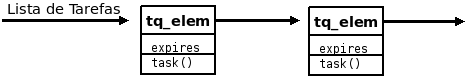
\includegraphics[scale=.8]{figs/task}
	\caption{Fila de tarefas agendadas do MIPL}
	\label{f_mipl_tasks}
\end{figure}

A \textit{thread runner}, fica percorrendo a fila de tarefas(ver figura
\ref{f_mipl_tasks}) e quando o tempo da tarefa expira, executa uma fun��o
associada, previamente registrada.

\subsubsection{\textit{icmp6\_listen}}
O MIPL cria uma \textit{thread} para escutar mensagens ICMPv6 e para isso cria
um soquete bruto. Por�m, h� muitas mensagens ICMPv6, por isso, para reduzir o
n�mero de pacotes passados do \textit{kernel} para a aplica��o, � fornecido um
filtro especifico pela aplica��o. Na tabela \ref{t_mipl_icmp} � poss�vel
observar as mensagens ICMPv6 que ser�o tratadas pelo MIPL.

\begin{table}[!htpb]
\centering
\begin{small}
  \setlength{\tabcolsep}{3pt}
\begin{tabular}{|c|c|c|c|}\hline
\raisebox{1.5ex}{Fun��o mip6d} & \raisebox{1.5ex}{Mensagem Filtrada} &
\raisebox{1.5ex}{Fun��o}\\ \hline
N� M�vel & ND\_ROUTER\_ADVERT & An�ncio de roteadores  \\ 
	 & ND\_NEIGHBOR\_ADVERT & An�ncio de vizinhan�a \\ 
	 & MIP\_HA\_DISCOVERY\_REPLY & Resposta de descoberta de agente
domiciliar \\
	 & ICMP6\_PARAM\_PROB & askdfj;al \\
	 & ICMP6\_DST\_UNREACH & Destino inalcan��vel \\ \hline
Agente Domiciliar & MIP\_PREFIX\_SOLICIT & Solicita��o de prefixo \\
		  & MIP\_HA\_DISCOVERY\_REQUEST & Descoberta de agente
domiciliar \\
		  & ND\_ROUTER\_ADVERT & An�ncio de roteadores \\
		  & ICMP6\_DST\_UNREACH & Destino inalcan��vel; \\ \hline
\end{tabular} 
\end{small}
\caption{Filtros para os pacotes ICMPv6 feitos pelo MIPL}
\label{t_mipl_icmp}
\end{table} 

Durante a execu��o do \textit{daemon} � feita a instala��o de manipuladores, que
tratam as mensagens, em uma lista global. Ao receber uma das mensagens ICMPv6
filtradas, a \textit{thread} percorre a lista de manipuladores e chama a fun��o
para tratar a mensagem.

\begin{figure}[!htpb]
	\centering
	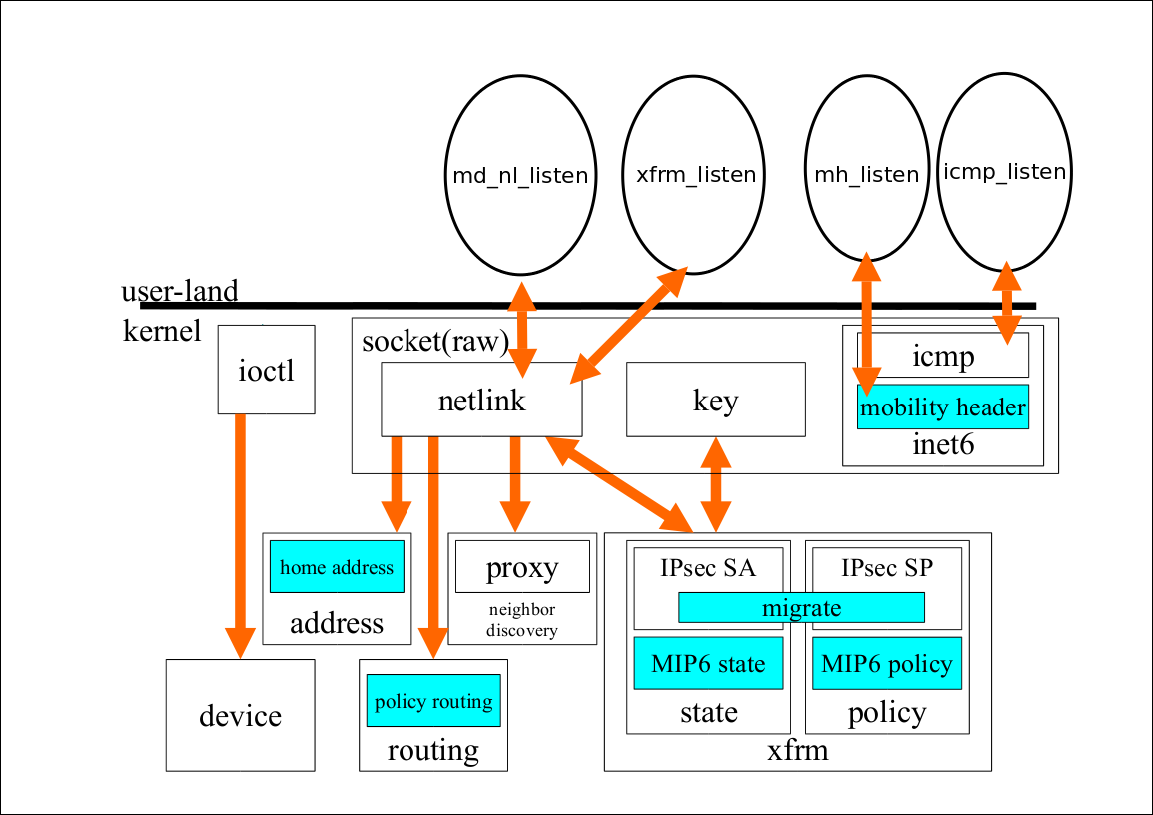
\includegraphics[scale=.27]{figs/mipl_kernel_block}
	\caption{Interfaces utilizadas pelo MIPL para fazer a comunica��o com o
kernel\cite{CitarFigura}}
	\label{f_mipl_kernel_blocks}
\end{figure}

\subsubsection{\textit{mh\_listen}}
\textit{Thread} criada para escutar a chegada de pacotes IPv6 com cabe�alho de
mobilidade. O seu funcionamento � semelhante a \textit{thread icmp6\_listen}: ao
receber uma mensagem com o cabe�alho de mobilidade chama um manipulador,
previamente instalado em uma lista global, para tratar a mensagem.

\subsubsection{\textit{xfrm\_listen}}
O \textit{daemon} cria a \textit{thread xfrm\_listen} que escuta mensagens
\textit{netlink} do \textit{framework} XFRM. Um manipulador � instalado para
tratar essas mensagens. As mensagens s�o: XFRM\_MSG\_ACQUIRE e
XFRM\_MSG\_REPORT.

\subsubsection{\textit{md\_nl\_listen}}
O \textit{mip6d} cria uma \textit{thread} para tratar mensagens \textit{netlink}
do tipo NETLINK\_ROUTE enviadas pelo \textit{kernel}. Esta \textit{thread} �
executada somente no n� m�vel.

A \textit{thread} ao receber uma mensagem \textit{netlink}, chama o manipulador
instalado para trat�-la. As mensagens tratadas pelo manipulador s�o as que
informam:
\begin{itemize}
 \item a interface ou liga��o: ligado ou desligado;
 \item as mudan�as no estado da alcan�abilidade do roteador padr�o;
 \item os \textit{Care-of-address} novos ou removidos.
\end{itemize}

\subsubsection{\textit{vt\_server\_recv}}
� possivel habilitar em tempo de compila��o um terminal virtual. O terminal
virtual permite que os usu�rios se conectem ao \textit{daemon}, via protocolo
\textit{telnet}, para obter informa��es sobre o MIPv6, por exemplo:
\begin{itemize}
 \item O tempo de vida do prefixo do agente domiciliar;
 \item O estado do \textit{Binding cache};
 \item A Lista de \textit{Bindig Updates}.
\end{itemize}

A \textit{thread} \textit{vt\_server\_recv} � criada para responder as conex�es
para o terminal virtual, que � executado na porta 7777.

\subsubsection{\textit{sigh}}
O \textit{mip6d} implementa uma \textit{thread} que � respons�vel por fazer o
tratamento de alguns sinais do sistema. Os sinais que passam a ser tratados pela
aplica��o s�o:
\begin{description}
 \item[SIGHUP:] Significa o reinicio do programa, o \textit{daemon} ao receber
esse sinal executa a fun��o \textit{reinit};
\item[SIGINT:] Causa a interrup��o do programa, em termos pr�ticos � o sinal
recebido quando se pressiona as teclas \textit{Control+C}. Neste caso ao receber
este sinal o \textit{daemon} chama a fun��o \textit{terminate};
\item[SIGTERM:] Solicita��o de t�rmino do programa, neste caso o \textit{daemon}
tamb�m chama a fun��o \textit{terminate}.
 \end{description}

� de extrema import�ncia o tratamento destes sinais pelo \textit{daemon}, pois
ao finalizar o programa � preciso deletar eventuais endere�os IP's, t�neis,
tabelas de roteamento.

\subsection{Detec��o de Movimento}
O algoritmo de detec��o de movimento do MIPL � inteiramente baseado na escuta
das mensagens de an�ncio de roteadores. O n� m�vel est� constantemente escutando
as mensagens de RA, sendo que o n� percebe o movimento quando:
\begin{itemize}
 \item o seu roteador padr�o torne-se inalcan��vel; para tanto, o n� m�vel de
tempos em tempos, verifica o roteador com um \textit{Neighbor Solicitation};
 \item passa a receber mensagens de outro roteador e para de escutar
mensagens do anterior.
\end{itemize}

Embora o MIPL seja uma extens�o da pilha IPv6 padr�o do \textit{Linux},
apresenta algumas caracter�sticas sobre administra��o de roteadores:
\begin{enumerate}
 \item O MIPL possui a sua pr�pria lista de roteadores. Esta lista cont�m o 
atual roteador de acesso, bem como roteadores que n�o s�o atualmente
utilizados, mas com tempo de vida n�o expirados;
 \item o MIPL for�a atualiza��es na tabela de roteamento ap�s receber um an�ncio
de novo roteador, e apaga todas as informa��es de roteamento que n�o s�o do
prefixo atual.
\end{enumerate}
Devido a estas duas caracter�sticas, o MIPL sempe escolhe um novo roteador. Este
m�todo de sele��o agressiva de roteadores traz uma melhora na detec��o de 
movimento, ou seja, no tempo de \textit{handover}.

\section{Altera��es no MIPL para obter o HMIPv6}
A primeira implementa��o necess�ria foi dar suporte ao MIPL a leitura das
mensagens RA divulgadas pelos MAP's, pois s�o elas que permitem a cria��o do
endere�o RCoA. No manipulador de mensagens RA foi adicionado o suporte para
a leitura da op��o de MAP na mensagem RA. Foi criada uma estrutura de dados
para o MAP e fun��es para manipula��o desta estrutura. Na estrutura de dados do
roteador foi adicionado uma lista de MAP's. A estrutura � mostrada a seguir.

\begin{lstlisting}
struct map_list_entry
{
    struct list_head list;
    struct timespec timestamp;
    struct tq_elem tqe;
    struct nd_opt_map map;
    struct in6_addr rcoa;
    int used;
};
\end{lstlisting}
A estrutura cont�m:
\begin{itemize}
 \item os campos da op��o de MAP da mensagem RA;
 \item tempo de vida do roteador que entregou a mensagem;
 \item endere�o RCoA criado a partir do endere�o do MAP;
 \item estrutura de dados que permite criar tarefas para serem agendadas;
\end{itemize}

No processamento da mensagem RA foram adicionados novos eventos de
movimento:\textbf{ME\_MAP\_NEW}, \textbf{ME\_MAP\_UPDATE} e
\textbf{ME\_MAP\_EXPIRED} Estes eventos tem a fun��o de colher os
dados que ser�o utilizados no momento do registro e  manter os dados para o
funcionamento do protocolo.

Foi criada tamb�m uma estrutura de dados para o RCoA tendo sido adicionada na
estrutura do agente domiciliar. As informa��es contidas na estrutura ser�o
utilizadas no momento da forma��o das mensagens de BU e no controle do registro.

\begin{lstlisting}
struct rcoa_addr_info {
    struct mn_addr rcoa; /* Home address for MAP */
    uint8_t mlen;
    uint8_t map_reg_status;
    struct in6_addr map_prefix;
    struct in6_addr map_addr;
    int pend_ba;
    int site;
    int if_tunnel;
};
\end{lstlisting}

Outas implementa��es foram realizadas no n� m�vel, quais sejam:
\begin {itemize}
 \item  foi acrescentado ao mecanismo de registro, um suporte ao envio do BU
para o MAP;
\item altera��o da mensagem de BU para o agente domiciliar;
\item cria��o do t�nel, com o MAP;
\item e modifica��o do t�nel com o agente domiciliar.
\end {itemize}

Algo interessante de salientar � que toda a parte de tomada de decis�o sobre o
movimento se manteve e as altera��es atuam somente na forma do registro com
os agentes.

\subsection{Detalhes do funcionamento}
A seguir, uma descri��o das implementa��es efetuadas no MIPL em um movimento
para um novo dom�nio:
\begin{enumerate}
 \item Ao receber uma mensagem RA de um novo roteador de acesso:
\begin{itemize}
 \item as op��es de MAP s�o lidas;
 \item uma lista de MAP's � criada na estrutura do roteador.
\end{itemize}
 \item Um novo MAP dispara um evento de movimento do tipo \textbf{ME\_MAP\_NEW}
que:
\begin{itemize}
 \item faz escolha de um MAP na lista de roteadores, baseado na dist�ncia em
saltos do MAP;
 \item cria um t�nel para o MAP;
 \item adiciona o RCoA na interface do t�nel;
 \item define o RCoA na estrutura do agente domiciliar, utilizado no envio do
BU.
\end{itemize}
 \item o movimento � detectado, usando o c�digo normal do MIPL. O registro
deve ser, ent�o, realizado com os agentes:
\begin{itemize}
 \item enviado BU para o MAP com os campos:
\begin{itemize}
 \item Origem = RCoA
 \item Destino = endere�o MAP
 \item Care-of-Adress = LCoA
\end{itemize}
 \item enviado BU para agente domiciliar com os campos:
 \begin{itemize}
  \item Origem = endere�o domiciliar
  \item Destino = endere�o agente domiciliar
  \item Care-of-Adress = RCoA
 \end{itemize}
\end{itemize}
 \item Ap�s o envio dos BU's, os t�neis devem ser modificados:
 \begin{itemize}
  \item T�nel entre n� m�vel e MAP: o ponto final � a interface de rede.
  \item T�nel entre n� m�vel e agente domiciliar: o ponto final � o t�nel entre
n� m�vel e MAP.
 \end{itemize}
 \item Periodicamente, com a chegada dos RA's, o evento de movimento
\textbf{ME\_MAP\_UDATE} � disparado e o tempo de vida do RCoA � atualizado.
\end{enumerate}

\subsection{Problemas conhecidos}
Considerando o car�ter experimental do trabalho, a disponibilidade de tempo
para a sua execu��o e a alta
complexidade do c�digo do MIPL, pode-se dizer que muito trabalho deve ainda ser
realizado para a obten��o de uma vers�o completa do HMIPv6. No que se refere a
implementa��o efetuada, alguns problemas podem, em particular, ser apontados:
\begin{itemize}
 \item aus�ncia de suporte a otimiza��o de rotas;
 \item aus�ncia de suporte a seguran�a (IPSec);
 \item aus�ncia de suporte ao HMIPv6 em arquivo de configura��o, somente em
tempo de compila��o;
 \item sem tarefas para deletar MAP's expirados;
 \item problema ao receber BA provindo do MAP, o que ocasiona problemas em
mobilidade em um mesmo dom�nio;
 \item problemas no retorno para rede domiciliar.
\end{itemize}

% ----------------------------------------------------------------------- %
% Arquivo: cenarios.tex
% ----------------------------------------------------------------------- %

\chapter{Cen�rios de Testes}

\section{Introdu��o}
Ap�s os estudos bibliogr�ficos sobre o protocolo MIPv6 e a prepara��o da Plataforma
 de Testes para Mobilidade, iniciou-se a etapa de defini��o e implementa��o de cen�rios
 com fins de analisar as funcionalidade dos protocolos.

Para analisar alguns mecanismos do protocolo e testar seus modos de opera��o, dois 
 cen�rios base foram definidos. Nesses dois cen�rios foi realizada tr�s simula��es.
 A primeira simula��o ocorre no cen�rio 1, descrito na figura \ref{f_cenario1}, onde
 � testado o modo de opera��o por tunelamento bi-direcional do MIPv6. A segunda simula��o
 tambem ocorre no cen�rio 1, sendo testado o modo de opera��o por otimiza��o de roteamento
 A terceira simula��o � no cen�rio 2, descrito na figura\ref{f_cenario2}, tendo como
 objetivo o funcionamento do HMIPv6.

%O computador que ser� utilizado para a realiza��o dos cen�rios de teste possui as seguintes 
% caracteristicas: \textit{Atlhon XP 2600}, 512MB de mem�ria e rodando \textit{Gnu/Linux 
% Slackware} 12.0, kernel linux-2.6.21.5.

Os arquivos para a configura��o dos cen�rios usados no Guml4Mip est�o dispon�veis no
 diret�rio da documenta��o do projeto.

%Para auxiliar na gera��o de \textit{logs}, que tendem a enriquecer an�lise dos cen�rios, foram utilizadas as ferramentas
%\textit{tcpdump}, \textit{ping6} e \textit{gen}.

\section{Fundamentos para a An�lise dos Cen�rios}
  Na an�lise dos cen�rios estudados vamos localizar os seguintes aspectos:
\begin{itemize}
  \item a sequ�ncia e a natureza das mensagens trocadas entre os v�rios n�s. Neste
 aspecto, utilizaremos as sa�das geradas pelos programas \textit{tcpdump};
  \item as tabelas de roteamento e regras de roteamento analisadas em situa��es chave,
 por exemplo, antes e depois da mobilidade;
  \item aspectos de desempenho e perdas de pacotes. Sabemos das limita��es desta an�lise 
 em um ambiente virtual, mas esperamos obter dados relativos. Tamb�m confrontaremos os dados
 obtidos com os resultados esperados segundo uma abordagem anal�tica.
  \item A cria��o e a manipula��o dos tuneis entre o agente domiciliar e o n� m�vel antes
 e depois do movimento.
\end{itemize}

\subsection{Tempo de lat�ncia do \textit{Handover}}
O processo de \textit{handover} acontece quando o n� m�vel muda seu ponto de conex�o 
 de uma sub-rede para outra. O tempo de lat�ncia envolvido neste processo \cite{xavier}
 pode ser dividida em quatro fases:

\begin{enumerate}
 \item \textbf{Detec��o de Movimento (\textit{TD})}: Em um cen�rio real representaria
 o tempo do \textit{handover} na camada de enlace at� o primeiro \textit{Router Advertisement}.
 Como neste ambiente de testes n�o conseguimos simular a camada enlace n�o se pode precisar
 com a exatid�o a lat�ncia envolvida no processo. Por�m, para fins de estudo consideraremos
 para nosso cen�rio o tempo entre o �tlimo pacote do \textit{gen} recebido na rede
 domiciliar e o primeiro \textit{Router Advertisement} na rede visitada.

\begin{equation}
 TD = t1 - t0
\label{eq.td}
\end{equation}

\item \textbf{Configura��o do \textit{Care-of-address} (\textit{TA})}: Tempo que entre 
 o primeiro \textit{Router Advertisement} e o envio do \textit{Binding Update}.

\begin{equation}
 TA = t2 -t1
 \label{eq.ta}
\end{equation}

\item \textbf{Registro com agente domiciliar (\textit{TR})}: Intervalo de tempo entre
 o envio do \textit{Binding Update} ao agente domiciliar e o recebimento do
 \textit{Binding Acknowledgement}.

\begin{equation}
 TR = t3 - t2
 \label{eq.tr}
\end{equation}

\item \textbf{Otimiza��o de Roteamento (\textit{TO})}: Intervalo de tempo entre o envio
 das mensagens do \textit{Return Routability Procedure} e o recebimento do
 \textit{Binding Acknowledgement} do n� correspondente.

\begin{equation}
 TO = t4 - t3
 \label{eq.to}
\end{equation}

\end{enumerate}

Obviamente podemos calcular o tempo de lat�ncia do handover com a seguinte f�rmula:

\begin{equation}
 TH = TD + TA + TR + TO
 \label{eq.th}
\end{equation}

\section{Cen�rio 1}
\label{s_cenario1}
O primeiro cen�rio de teste � formado por tr�s redes interligadas entre si e cinco n�s. A sua topologia pode ser observada na figura \ref{f_cenario1}, onde o numero nos bal�es cinza representam a vlan no \textit{uml-switch}. Os endere�os atribu�dos as interfaces dos n�s, durante a realiza��o do cen�rio, bem como seus endere�os de hardware est�o dispon�veis na tabela \ref{t_addr1}.

\begin{figure}[!htpb]
	\centering
	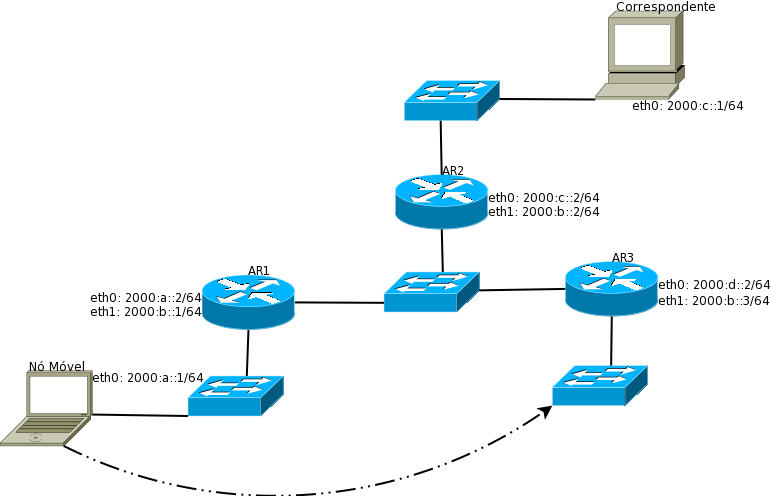
\includegraphics[scale=.4]{figs/cenario1}
	\caption{Topologia do Cen�rio 1}
	\label{f_cenario1}
\end{figure}


Na rede com prefixo 2000:a::/64 est� o n� correspondente com quem o n� m�vel est� se comunicando. Na rede com o prefixo
 2000:c::/64 est� presente um roteador (HA) que oferece o servi�o de agente domiciliar ao n� m�vel. A rede com prefixo
 2000:d::/64 � a rede que o n� m�vel deve visitar.

\begin{table}[!htpb]
\centering
\begin{small}
  \setlength{\tabcolsep}{3pt}
\begin{tabular}{|c|c|c|c|c|}\hline
\raisebox{1.5ex}{N�} & \raisebox{1.5ex}{Interface} & \raisebox{1.5ex}{MAC} & \raisebox{1.5ex}{Endere�o} & \raisebox{1.5ex}{Tipo}\\ \hline
% MN
& & & 2000:a::1 & Domiciliar (Global) \\ 
MN & eth0 & 92:09:4F:D5:EF:EA & 2000:a::9009:4fff:fed5:efea & Auto-configurado \\
& & & 2000:d::9009:4fff:fed5:efea & Care-of-address \\
& & & fe80::9009:4fff:fed5:efea & Local \\ \hline
% CN
CN & eth0 & D6:7F:B0:C3:C9:0C & 2000:c::1 & Global \\ 
& & & fe80::d47f:b0ff:fec3:c90 & Local \\ \hline
% AR1
& eth0 & AE:4D:A8:10:EB:1D & 2000:a::2 & Global \\ 
AR1 & & & fe80::ac4d:a8ff:fe10:eb1d & Local \\
& eth1 & 1E:2D:C8:43:E6:C7 & 2000:b::1 & Global \\ 
& & & fe80::1c2d:c8ff:fe43:e6c7 & Local \\ \hline
%AR2
& eth0 & 36:A7:3F:06:58:8D & 2000:c::2 & Global \\ 
AR2 & & & fe80::34a7:3fff:fe06:588d & Local \\ 
& eth1 & 4A:19:FD:12:48:34 & 2000:b::2 & Global \\
& & & fe80::4819:fdff:fe12:4834 & Local \\ \hline
%AR3
& eth0 & B2:4C:E9:EC:6C:42 & 2000:d::2 & Global \\ 
AR3 & & & fe80::b04c:e9ff:feec:6c42 & Local \\ 
& eth1 & 2A:E2:57:C7:4F:E4 & 2000:b::3 & Global \\
& & & fe80::28e2:57ff:fec7:4fe4 & Local \\ \hline
\end{tabular} 
\end{small}
\caption{Endere�os do Cen�rio 1}
\label{t_addr1}
\end{table} 


\subsection{Simula��o 1}

A simula��o 1 ter� a seguinte sequ�ncia. No in�cio o n� correspondente come�a a enviar mensagens ICMP por meio do \textit{ping6} para o n� m�vel.

\begin{verbatim}
cn# ping6 2001:a::2
\end{verbatim}

O n� m�vel realiza o monitoramento de todo o funcionamento do MIPv6 durante o processo de \textit{handover} utilizando o \textit{tcpdump} em o modo \textit{verbose} (-vvv) e para mostrar o conte�do do pacote em hexadecimal (-X).

\begin{verbatim}
mn# tcpdump -vvvX
\end{verbatim}

\subsubsection{Troca de Mesagens}
Os dados obtidos na sa�da do comando \textit{tcpdump} foram compilados em forma de uma tabela para facilitar a visualiza��o dos mesmos e podem ser observados na tabela \ref{t_resul_1}.
Analisando os dados recolhidos conseguimos observar exato momento que ocorreu a mobilidade para a outra rede. No instante entre o ICMP reply X e o RA recebido � o perio que o n� m�vel realiza o movimento.

\subsubsection{Tabelas de Roteamento}
Podemos constatar mudan�as nas tabelas de roteamento do n� m�vel e do agente domiciliar depois da mobilidade nas respecitivas figuras \ref{t_rot_mn1} e \ref{t_rot_ha1}, ap�s receber o \textit{Binding Update} e o agente domiciliar criar o t�nel com o n� m�vel, � adicionada a seguinte rota a sua tabela de roteamento, que todos os pacotes com destino ao endere�o domiciliar devem ser encaminhados para o t�nel. E no n� m�vel os pacotes com destino ao n� correspondente e ao agente domiciliar s�o encaminhados pelo t�nel, caracterizando o tunelamento bidirecional.

\subsubsection{Regras de Roteamento}

\subsubsection{Tuneis}


\begin{table}[!htpb]
\centering
\begin{small}
  \setlength{\tabcolsep}{3pt}
\begin{tabular}{|c|c|c|c|}\hline
\raisebox{1.5ex}{Destino} & \raisebox{1.5ex}{Via} & \raisebox{1.5ex}{Proximo salto} & \raisebox{1.5ex}{Considera��es}\\ \hline
default & eth0 & fe80::ac4d:a8ff:fe10:eb1d & Na rede domiciliar \\ \hline
default & eth0 & fe80::b04c:e9ff:feec:6c42 & \\ 
2000:a::2 & ip6tnl1 & 2000:a::2 & Na rede visitada \\ 
2000:c::1 & ip6tnl1 & 2000:c::1 & \\ \hline
\end{tabular} 
\end{small}
\caption{Tabela de roteamento do n� m�vel}
\label{t_rot_mn1}
\end{table} 

\begin{table}[!htpb]
\centering
\begin{small}
  \setlength{\tabcolsep}{3pt}
\begin{tabular}{|c|c|c|c|}\hline
\raisebox{1.5ex}{Destino} & \raisebox{1.5ex}{Via} & \raisebox{1.5ex}{Proximo salto} & \raisebox{1.5ex}{Considera��es} \\ \hline
2000:c::/64 & eth1 & 2000:b::2 &  Antes da mobilidade do n� m�vel \\ 
2000:d::/64 & eth1 & 2000:b::3 &   \\ \hline
2000:c::/64 & eth1 & 2000:b::2 & \\
2000:d::/64 & eth1 & 2000:b::3 & Ap�s a mobilidade do n� m�vel \\
2000:a::1 & ip6tnl1 & 2000:a::1 & \\ \hline
\end{tabular} 
\end{small}
\caption{Tabela de roteamento do agente domiciliar}
\label{t_rot_ha1}
\end{table} 

\begin{table}[!htpb]
\centering

\begin{small}
  \setlength{\tabcolsep}{3pt}
\begin{tabular}{|c|c|c|c|}\hline
\raisebox{1.5ex}{Tempo (s)} & \raisebox{1.5ex}{Origem} & \raisebox{1.5ex}{Destino} & \raisebox{1.5ex}{Conte�do}\\ \hline
21:59.952226 & fe80::ac4d:a8ff:fe10:eb1d & ff02::1 & RA, Flags [Home Agent]\\
22:00.525313 & fe80::ac4d:a8ff:fe10:eb1d & 2000:a::1 & NS, who 2000:a::1\\
22:00.525398 & 2000:a::1 & fe80::ac4d:a8ff:fe10:eb1d & Neighbor Advertisement\\
22:00.656486 & 2000:c::1 & 2000:a::1 & Gen seq\#=5\\ 
22:01.664448 & 2000:c::1 & 2000:a::1 & Gen seq\#=6\\ \hline
\textbf{22:03.467587} & \textbf{fe80::b04c:e9ff:feec:6c42} & \textbf{ff02::1} & \textbf{Router Advertisement}\\
22:03.482118 & :: & ff02::16 & HBH, multicast listener\\
22:03.799224 & :: & ff02::1:ffd5:efea & NS, who fe80::9009:4fff:fed5:efea\\
22:04.285049 & :: & ff02::1:ffd5:efea & NS, who 2000:d::9009:4fff:fed5:efea\\ 
\textbf{22:05.288026} & \textbf{2000:d::9009:4fff:fed5:efea} & \textbf{2000:a::2} & \textbf{BU seq\#=26356 AH}\\
22:05.304531 & fe80::9009:4fff:fed5:efea & ff02::16 & HBH, multicast listener\\
22:06.305532 & fe80::b04c:e9ff:feec:6c42 & ff02::1:ffd5:efea & NS, who 2000:d::9009:4fff:fed5:efea\\
22:06.305650 & 2000:d::9009:4fff:fed5:efea & fe80::b04c:e9ff:feec:6c42 & Neighbor Advertisement\\
\textbf{22:06.305972} & \textbf{2000:a::2} & \textbf{2000:d::9009:4fff:fed5:efea} & \textbf{BA seq\#=26356 lifetime=262140}\\
22:06.316950 & fe80::b04c:e9ff:feec:6c42 & ff02::1 & Router Advertisement\\
22:06.512529 & fe80::9009:4fff:fed5:efea & fe80::ac4d:a8ff:fe10:eb1d & NS, who fe80::ac4d:a8ff:fe10:eb1d\\
22:06.700567 & 2000:a::2 & 2000:d::9009:4fff:fed5:efea & 2000:c::1 > 2000:a::1 (Gen seq\#=11)\\
22:07.510304 & fe80::9009:4fff:fed5:efea & fe80::ac4d:a8ff:fe10:eb1d & NS, who fe80::ac4d:a8ff:fe10:eb1d\\
22:07.705972 & 2000:a::2 & 2000:d::9009:4fff:fed5:efea & 2000:c::1 > 2000:a::1 (Gen seq\#=12)\\
22:08.338339 & fe80::b04c:e9ff:feec:6c42 & ff02::1 & Router Advertisement\\
. & . & . & .\\
. & . & . & .\\
. & . & . & .\\
22:18.785859 & 2000:a::2 & 2000:d::9009:4fff:fed5:efea & 2000:c::1 > 2000:a::1 (Gen seq\#=23)\\ \hline
\textbf{22:19.815983} & \textbf{fe80::ac4d:a8ff:fe10:eb1d} & \textbf{ff02::1} & \textbf{RA, Flags [Home Agent]}\\
22:19.839337 & :: & ff02::16 & HBH, multicast listener\\
22:19.877057 & :: & ff02::16 & HBH, multicast listener\\
22:20.170279 & :: & ff02::1:ffd5:efea & NS, who 2000:a::9009:4fff:fed5:efea\\
22:20.585230 & :: & ff02::1:ffd5:efea & NS, who fe80::9009:4fff:fed5:efea\\
22:20.879643 & :: & ff02::16 & HBH, multicast listener\\
22:21.585309 & :: & ff02::1:ff00:1 & NS, who 2000:a::1\\
22:21.606725 & fe80::9009:4fff:fed5:efea & ff02::16 & HBH, multicast listener\\
22:21.767709 & fe80::ac4d:a8ff:fe10:eb1d & ff02::1 & Neighbor Advertisement\\
\textbf{22:21.772629} & \textbf{2000:a::1} & \textbf{2000:a::2} & \textbf{BU seq\#=26357}\\
22:21.785931 & fe80::9009:4fff:fed5:efea & ff02::16 & HBH, multicast listener \\
22:21.792882 & fe80::ac4d:a8ff:fe10:eb1d & ff02::16 & HBH, multicast listener \\
22:21.812524 & fe80::ac4d:a8ff:fe10:eb1d & ff02::1:ff00:1 & NS, who 2000:a::1 \\
22:21.812620 & 2000:a::1 & fe80::ac4d:a8ff:fe10:eb1d & Neighbor Advertisement \\
22:21.812932 & 2000:c::1 & 2000:a::1 & Gen seq\#=27 \\
\textbf{22:21.874997} & \textbf{2000:a::2} & \textbf{2000:a::1} & \textbf{BA seq\#=26357 lifetime=0} \\
22:21.904397 & 2000:a::1 & ff02::1 & Neighbor Advertisement \\
22:22.569757 & fe80::ac4d:a8ff:fe10:eb1d & ff02::1 & RA, Flags [Home Agent] \\
22:22.814652 & 2000:c::1 & 2000:a::1 & Gen seq\#=28 \\ \hline
\end{tabular} 
\end{small}
\caption{Mensagens do Cen�rio 1 com Tunelamento Bidirecional}
\label{t_resul_1}
\end{table} 


\begin{table}[!htpb]
\centering
\begin{small}
  \setlength{\tabcolsep}{3pt}
\begin{tabular}{|c|c|c|c|}\hline
\raisebox{1.5ex}{Tempo (s)} & \raisebox{1.5ex}{Origem} & \raisebox{1.5ex}{Destino} & \raisebox{1.5ex}{Conte�do}\\ \hline
50:21.991721 & 2000:a::1 & 2000:c::1 & ICMP6, echo reply \\ \hline
\textbf{50:24.231519} & \textbf{fe80::b04c:e9ff:feec:6c42} & \textbf{ff02::1} & \textbf{Router Advertisement}\\
50:24.247992 & :: & ff02::16 & HBH, multicast listener\\
50:24.545598 & :: & ff02::1:ffd5:efea & NS, who 2000:d::9009:4fff:fed5:efea\\ 
50:24.879467 & :: & ff02::1:ffd5:efea & NS, who fe80::9009:4fff:fed5:efea\\
50:25.548165 & fe80::b04c:e9ff:feec:6c42 & ff02::1 & Router Advertisement\\
\textbf{50:25.557223} & \textbf{2000:d::9009:4fff:fed5:efea} & \textbf{2000:a::2} & \textbf{BU seq\#=47808 AH}\\
50:25.576407 & :: & ff02::16 & HBH, multicast listener\\
50:26.581135 & fe80::b04c:e9ff:feec:6c42 & ff02::1:ffd5:efea & NS, who 2000:d::9009:4fff:fed5:efea\\
50:26.581276 & 2000:d::9009:4fff:fed5:efea & fe80::b04c:e9ff:feec:6c42 & Neighbor Advertisement\\
\textbf{50:26.581588} & \textbf{2000:a::2} & \textbf{2000:d::9009:4fff:fed5:efea} & \textbf{BA seq\#=47808 lifetime=262140}\\ \hline
50:26.987535 & fe80::9009:4fff:fed5:efea & fe80::ac4d:a8ff:fe10:eb1d & NS, who fe80::ac4d:a8ff:fe10:eb1d\\
50:27.009344 & 2000:a::2 & 2000:d::9009:4fff:fed5:efea & 2000:c::1 > 2000:a::1, (icmp6)\\
50:27.009538 & 2000:d::9009:4fff:fed5:efea & 2000:a::2 & 2000:a::1 > 2000:c::1,(icmp6)\\
\textbf{50:27.013543} & \textbf{2000:d::9009:4fff:fed5:efea} & \textbf{2000:a::2} & \textbf{2000:a::1 > 2000:c::1,(HoTI)}\\
\textbf{50:27.015165} & \textbf{2000:d::9009:4fff:fed5:efe} & \textbf{2000:c::1} & \textbf{CoTI Care-of Init}\\
\textbf{50:27.019919} & \textbf{2000:a::2} & \textbf{2000:d::9009:4fff:fed5:efea} & \textbf{2000:c::1 > 2000:a::1, (HoT)}\\
\textbf{50:27.029192} & \textbf{2000:c::1} & \textbf{2000:d::9009:4fff:fed5:efea} & \textbf{CoT}\\
\textbf{50:27.031650} & \textbf{2000:d::9009:4fff:fed5:efea} & \textbf{2000:c::1} & \textbf{BU seq\#=1077 A}\\
\textbf{50:27.037401} & \textbf{2000:c::1} & \textbf{2000:d::9009:4fff:fed5:efea} & \textbf{BA seq\#=1077 lifetime=420}\\
50:27.365152 & fe80::b04c:e9ff:feec:6c42 & ff02::1 & Router Advertisement\\
50:27.982719 & fe80::9009:4fff:fed5:efea & fe80::ac4d:a8ff:fe10:eb1d & Neighbor Solicitation\\
50:28.014358 & 2000:c::1 & 2000:d::9009:4fff:fed5:efea & ICMP6, echo request\\
50:28.014494 & 2000:d::9009:4fff:fed5:efea & 2000:c::1 & ICMP6, echo reply \\ \hline
\end{tabular} 
\end{small}
\caption{Mensagens do Cen�rio 1 com Otimiza��o de Roteamento}
\label{t_mes_ro}
\end{table} 

Na tabela \ref{t_handover}, encontram-se os tempos das fases do processo de \textit{handover} referentes ao cen�rio estudado.

\begin{table}[!htpb]
\centering
\begin{small}
  \setlength{\tabcolsep}{3pt}
\begin{tabular}{|c|c|c|}\hline
\raisebox{1.5ex}{Fase} & \raisebox{1.5ex}{Tempo (ms)} & \raisebox{1.5ex}{Media \%} \\ \hline
\textit{TD} & 2240 & 48,6 \\ \hline
\textit{TA} & 1320 & 28.63\\ \hline
\textit{TR} & 1030 & 22.34\\ \hline
\textit{TO} & 20 &  0.43\\ \hline
\textit{TH} & 4610 & 100 \\ \hline
\end{tabular} 
\end{small}
\caption{Lat�ncia no \textit{Handover} do cen�rio estudado}
\label{t_handover}
\end{table} 

Utilizando o cen�rio estudado como refer�ncia, foi realizado um teste que pretende verificar a perda na taxa de transmiss�o em um processo de \textit{handover}. Utilizando a ferramenta \textit{gen} que permite gerar tr�fegos espec�ficos e relat�rios que extraem a taxa de trasmiss�o e a perda de pacotes, e utilizando o utilit�rio \textit{GNUPLOT} somos capazes de gerar gr�ficos que avaliam esse desempenho.

Os testes realizados foram feitos utilizando tunelamento bidirecional, o tempo configurado para o intervalo entre as mensagens de \textit{Router Advertisement} foi de 30 � 70 milisegundos. Os comandos disparados nos n�s m�vel e correspondente foram os seguintes:
\begin{verbatim}
mn# gen -l -d -p udp -s 14000 -f /host/log/
cn# gen -a 2000:a::1 -d -p udp -s 14000
\end{verbatim}

O gr�fico obtido no teste, pode ser observado na figura \ref{f_banda}.

\begin{figure}[!htpb]
	\centering
	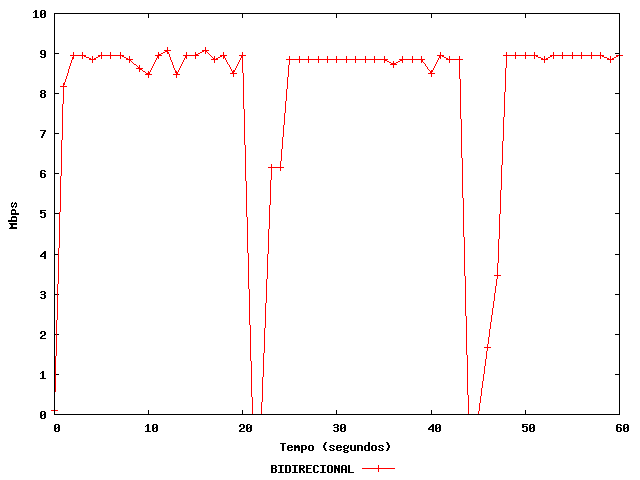
\includegraphics[scale=.6]{figs/banda}
	\caption{Taxa de transmiss�o em \textit{Handover}}
	\label{f_banda}
\end{figure}

A partir dos dados levantados com o teste podemos tirar v�rias conclus�es, entre as quais destacam-se que o \textit{Troughput} suportado pela rede gira em torno de 9 Mbps, este dado esta muito relacionado ao desempenho da m�quina hospedeiro, que cada \textit{handover} � de aproximadamente 3 segundos, h� perdas consider�veis de pacotes que prejudicariam muito comunica��es interativas como videoconfer�ncia e \textit{VoIP}, por�m, navega��o em paginas da \textit{Internet} e visualiza��o de \textit{e-mail} a instabilidade � toler�vel.

Como cen�rio estudo foi simulado todos os tempos medidos s�o estimados. Por�m, segundo algumas bibliografias estudadas que realizaram experimentos fisicamente os tempos medidos na simula��o est�o dentro do esperado.

� percept�vel que as fases que mais comprometem o \textit{handover} do nosso cen�rio s�o as da detec��o de movimento e a configura��o do \textit{care-of-address}. Algumas tentativas podem ser feitas para tentar diminuir a lat�ncia nestas duas fases.

Na tentativa de diminuir o tempo da fase de detec��o de movimento, podemos diminuir o intervalo entre as mensagens de \textit{Router Advertisement} do roteador presente na rede que ir� ser visitada pelo n� m�vel. Pois, � por meio desta mensagem que o n� m�vel detecta o movimento e desencadeia todo o processo de \textit{handover}.

No intuito de verificar se h� uma melhora no processo de handover. O cen�rio estudado foi repetido variando o intervalo entre as mensagens de \textit{Router Advertisement}. O resultado deste teste esta dispon�vel na figura \ref{f_radvd}.

\begin{figure}[!htpb]
	\centering
	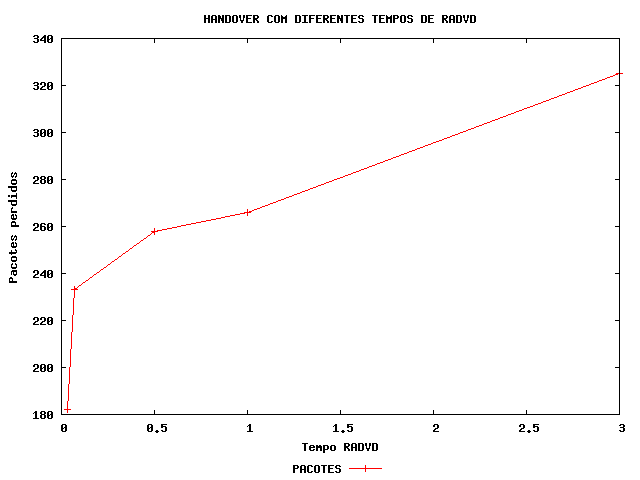
\includegraphics[scale=.6]{figs/radvd}
	\caption{Diferentes intervalos entre as mensagens \textit{Router Advertisement}}
	\label{f_radvd}
\end{figure}

Com os dados levantados, � poss�vel perceber que o intervalo entre as mensagens de \textit{Router Advertisement} esta diretamente ligado com a perda de pacotes durante o \textit{handover}. Por�m, esta n�o � uma boa pr�tica para tentar amenizar a lat�ncia do handover, pois um numero muito grande de mensagens \textit{multicasting} inundaria a rede prejudicando a perfomance principalmente em redes sem fio.

No processo de forma��o de um novo \textit{care-of-address} o DAD � necess�rio para se certificar que o endere�o formado � exclusivo. Para o teste ser bem sucedido nenhum n� vizinho deve enviar um \textit{Neighbor Advertisement}, em resposta ao teste, ou \textit{Neighbor Solicitation}, como o mesmo endere�o em quest�o, em um per�odo de \textit{1000ms} segundo a RFC 2462 \cite{rfc2462}. Este tempo de espera compromete a fase de configura��o do \textit{care-of-address}.

Existe uma vari�vel chamada \textit{dad\_transmits} no kernel do Linux que � usada para configurar o DAD em um n�. Com a inten��o de diminuir a lat�ncia na fase de configura��o do \textit{care-of-address}, n�s configuramos a vari�vel com o valor 0, isso significa que o procedimento de DAD � cancelado, e repetimos o cen�rio estudado.

\section{Resultados}
Com a realiza��o dos experimentos podemos constatar o funcionamento do protocolo e perceber continua��o da comunica��o entre os pontos comunicantes ap�s a mobilidade de forma transparente as camadas superiores a de rede, observar todas as mensagens trocadas no processo e estimar o tempo de lat�ncia com a mobilidade.
O primeiro resultado que se pode obter com a realiza��o do Cen�rio 1, foi o perfeito funcionamento do MIPv6, ocorreram algumas perdas de pacotes, mas o n� m�vel conseguiu continuar sendo alcan�ado pelo seu endere�o domiciliar mesmo n�o estando em sua rede domiciliar.

\section{Cen�rio 2}
\label{s_cenario2}


\begin{figure}[!htpb]
	\centering
	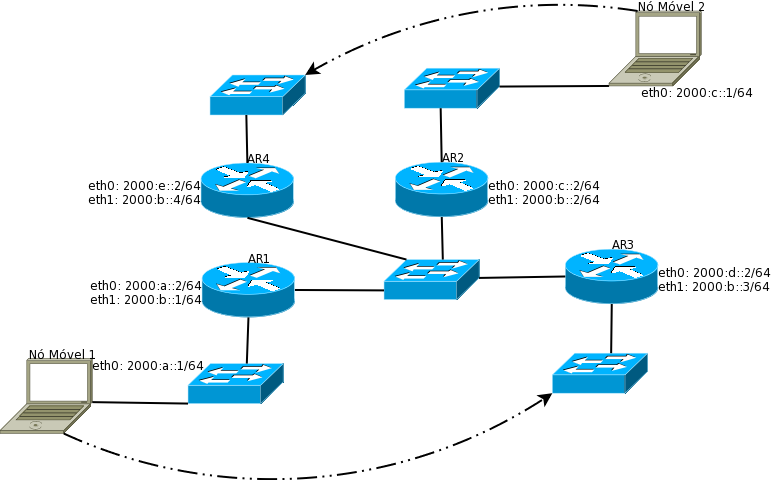
\includegraphics[scale=.37]{figs/cenario2}
	\caption{Topologia do Cen�rio 2}
 	\label{f_cenario2}
\end{figure}

\section{Conclus�o}

\frame{
\frametitle{Conclus�o}

\begin{itemize}
\item A platarfoma implementada possibilita:
\begin{itemize}
 \item Realizar mobilidade entre sub-redes, devido a implementa��o
realizada no \textit{switch} virtual;
 \item Constru��o e realiza��o facilitada de cen�rios de mobilidade;
 \item Utiliza��o sem conhecimentos espec�ficos obre as m�quinas virtuiais
UML, compila��o do \textit{kernel linux} e dos \textit{daemons} dos protocolos;
 \item Ser utilizada para outros estudos sobre redes de computadores, 
mostrando-se flex�vel.
\end{itemize}
\item A plataforma de testes  atingiu o objetivo desejado e vem 
demonstrando bons resultados.

\end{itemize}

}

\frame{
\frametitle{Conclus�o}

\begin{itemize}
\item Foi gerado uma vers�o experimental do HMIPv6.
\item  Mesmo n�o tendo alcan�ado uma vers�o completa do protocolo, a realiza��o
do trabalho contribui para o enriquecimento de v�rios conhecimentos.
\begin{itemize}
\item Linguagem de programa��o C
\item Desenvolvimento em sistemas \textit{linux}
\item Kernel \textit{linux}
\item API de soquetes IPv6
\item POSIX \textit{Threads}.
\end{itemize}
\end{itemize}

}




\frame{
\frametitle{Trabalhos Futuros(Plataforma)}

\begin{itemize}
\item Concep��o de um simulador da rede sem fio nas m�quinas UML, de forma
similar ao MobUML, possibilitando a an�lise dos problemas associados ao enlace e
seus impactos na camada de rede.
\item Implementa��o de modelos de mobilidade cl�ssicos, de forma a produzir
movimentos circulares, retil�neos, randomizados, ou mesmo, a acoplagem a um
simulador de movimentos urbanos, tal como o
\textit{Simulation of Urban MObility}.
\item Incrementos na linguagem de descri��o da UML, de forma a incorporar
aspectos de configura��o do IPv4 e facilitar a incorpora��o de novos protocolos
e \textit{deamons}.
\end{itemize}

}

\frame{
\frametitle{Trabalhos Futuros(Plataforma)}
\begin{itemize}
\item Melhorias na configura��o dos terminais virtuais e consoles, de forma a
obter Uma melhor visualiza��o do sistema por parte do usu�rio.
\item Desenvolvimento de uma interface gr�fica para a configura��o das
m�quinas UML.
\item Cria��o autom�tica de uma conex�o virtual entre a m�quina hospedeira e
as m�quinas virtuais.
\item Melhorias no instalador do sistema.
\end{itemize}
}

\frame{
\frametitle{Trabalhos Futuros(Extens�es MIPLs)}
\begin{itemize}
\item Implementa��o da otimiza��o de rotas no HMIP, ou seja, a realiza��o de
BUs diretamente com os n�s correspondentes;
\item Explora��o da implementa��o do HMIP para estudar melhorias na sele��o de
MAPs por parte dos n�s m�veis;
\item Estudo da integra��o do HMIP com protocolos de sinaliza��o de QoS,
desenvolvendo m�dulos/bibliotecas para o interfaceamento entre eles;
\item Incorpora��o do protocolo FMIPv6(rfc4068) na plataforma de
mobilidade;
\end{itemize}
}




\frame{
\frametitle{Bibliografia}
	% estilo para aparecer um icone de um livro
	%\beamertemplatebookbibitems
	% estilo para aparecer um icone de um paper =)
	\beamertemplatearticlebibitems
	\begin{thebibliography}{1}

	\bibitem{rfc3775}
	JOHNSON, D. ; PERKINS, C.; ARKKO, J.
	\newblock{\em Mobility Support in IPv6. RFC 3775}
	\newblock{\url http://www.ietf.org/rfc/rfc3775.txt}

	\bibitem{rfc4140}
	SOLIMAN, H.; CASTELLUCCIA, C.; EL MALKI, K.; BELLIER, L.
	\newblock {\em Hierarchical Mobile IPv6 Mobility Management, RFC 4140}
	\newblock{\url http://www.ietf.org/rfc/rfc4140.txt}

	\bibitem{rfc4068}
	KOODLI, R. 
	\newblock {\em Fast Handovers for Mobile IPv6, RFC 4068}
	\newblock{\url http://www.ietf.org/rfc/rfc4068.txt}
	
	\bibitem{mipl}
	NUORVALA, V.; PETANDER, H.; TUOMINEN,
	\newblock MIPL PROJECT. Mobile IPv6 for Linux, Version 2.0 RC1. 2004
	\end{thebibliography}
}

\end{document}
